\documentclass[a4paper]{article}

\usepackage[english]{babel}
\usepackage[utf8]{inputenc}
\usepackage{amsmath}
\usepackage{graphicx}
\usepackage[colorinlistoftodos]{todonotes}
\usepackage{pdfpages}

\title{Concepts Avancés de Bases de données}

\author{Joaquim LEFRANC et Jérôme Skoda}

\date{\today}

\begin{document}
\maketitle

\begin{abstract}
Comment avons nous pu écrire autant de chose sur seulement deux boucles imbriqués et une fonction de merge de moins de 20 lignes?
\end{abstract}

\section{Comment compiler le projet}

\subsection{Avec le terminal}

\begin{itemize}
	\item make all : Compile tout les fichiers
	\item make test : Lancement de la série de tests automatiques
	\item make doc  : Génération de la documentation (doxygen)
	\item make rapport : Génération du rapport (latex)
	\item make clean : Nettoyage du projet (supression des objets et binaires)
	\item make demo-tp1 : Lancer la démo tp1
	\item make demo-tp2 : Lancer la démo tp2
	\item make rm-rs : Supprime le fichier res/RS.txt
\end{itemize}

\subsection{Avec ECLIPSE}

Pour lancer une commande utiliser les boutons magique build targets.

\begin{figure}[h!] 
\centering
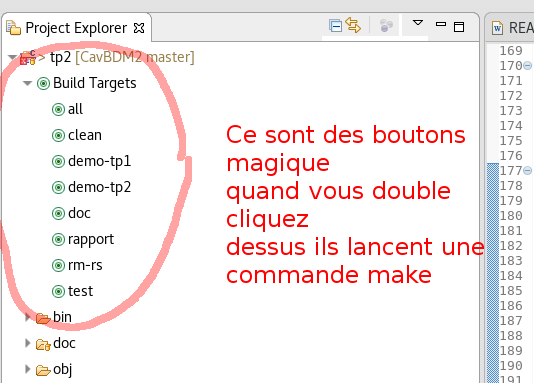
\includegraphics[width=0.5\textwidth]{bouton-magique.png}
\caption{Double clique ici!}
\end{figure}


\subsection{Avec code:block}

Aucun portage sur code:block de prévu. 
Nous avons passé une longue heure à configurer eclipse et nous en avons assez!

\section{Arborescence}

\begin{itemize}
\item bin : Binaire exécutable
\begin{itemize}
  \item demo : Exécutable de démonstration
  \item test : Exécutable de test
\end{itemize}
\item doc : Documentation doxygen sous differents formats
\item rapport : Source du rapport
\item res : Ressources necessaire au projet (fichier de bdd)
\item script  : Script utilisé pour les test
\item src : Source du projet
\begin{itemize}
  \item bdd   : Source de la bibliothéque
  \item demo  : Sources des differentes démonstrations d'utilisation
  \item test  : Sources des dufferents tests
\end{itemize}

\item sujet.pdf  : Sujet du projet
\item README.md  : Le readme du projet 
\item rappot.pdf : C'est moi
\end{itemize}

\section{Caracteristiques}

\begin{itemize}
	\item Le code est organisé
	\item Il y a des code des tests
	\item Il y a la doc
	\item Il y a un rapport
	\item Et il y a pleins d'autre chose
\end{itemize}

\section{Test unitaire}


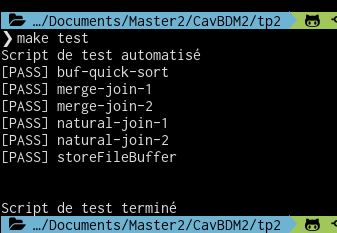
\includegraphics[width=0.8\textwidth]{test.png}



\includepdf[pages=3-12]{refman.pdf}

\end{document}
              
